\section{Foundational Markovian transport theories} 

\subsection*{Einstein's 1937 Thesis: the dispersion of bed load grains} 

Before 1937 Einstein added colored stones to an artificial stream channel and investigated their movement characteristics downstream \citep{Einstein1937}. 
He subsequently developed a probabilistic model describing the statistics of downstream particle travel distance with time. 
In this way he derived that particle travel distance with time should be a Poisson distribution. 
Einstein's introduction justifies his probabilistic approach: 
\begin{quote}
The (experimental) results demonstrated clearly that even under the same experimental conditions stones having essentially identical characteristics were transported widely varying distances ... (yet) similar curves were obtained when one plotted the frequency of particles as a function of the path. 
Consequently, it seemed reasonable to approach the subject of particle movement as a probability problem.  
\end{quote} 

Einstein's model, developed for low transport rates, has three key assumptions: (1) sediment motion is an alternating series of rest and motion intervals; (2) rest and motion can be characterized by random variables governed by probability distributions; and (3) because the time spent in motion is small relative to the time spent at rest, motion can be considered instantaneous. 
Within this conceptual picture, particle motions trace out stair step trajectories through the space time plane. 
Some example trajectories are indicated in \ref{fig:einsteinTrajectories}.
Although each trajectory is different, they define a probability distribution when many are collected. 

\begin{wrapfigure}{L}{0.5\textwidth}
  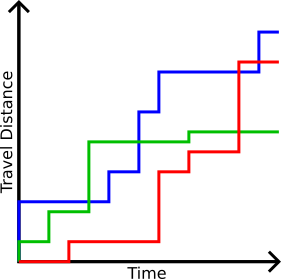
\includegraphics[width=.98\linewidth]{./figures/einsteintrajectories.png}
  \caption{The travel distance - time plane with three particle trajectories indicated as they were conceptualized by Einstein in terms of alternate start-stop motions. Each corner on the stair step trajectories is a transition between motion and rest states. The time spent at rest (resting time) and the distance traveled in motion (hop distance) are random variables drawn from probability distributions. These random motions coordinate so that motions are statistically described by a Poisson distribution.}
  \label{fig:einsteinTrajectories}
\end{wrapfigure}

Einstein considered that the random hop distances and travel times were described by exponential distributions: 
\begin{align}
P_L(l) &= l_0 e^{l/l_0} && \text{(hop distance)} \label{eq:hop}\\
P_T(t) &= T_0 e^{t/T_0} && \text{(travel time)} \label{eq:rest}
\end{align}
Here $l_0$ and $\tau_0$ are the mean hop distance and travel time, respectively.  
Einstein's key insight was that the distribution of downstream particle positions $P(x,t)$ at each space-time point $(x,t)$ can be computed as a path integral over all possible stair-step trajectories through the $(x,t)$ plane. 
Particle trajectories from $(0,0)$ to $(x,t)$ can differ in the number of steps, the height of each step (hop distance), and the width of each step (resting time). 
Einstein's argument to derive the resulting particle travel distance distribution is now briefly summarized. 

Consider that a large number of particles are released into the water stream at the space-time point $(x=0,t=0)$, so they are initially in a state of motion. 
Subsequently, these particles will transition to the resting state so the fraction of particles at each point $(x_0,t=0)$ is 
$$P(x = x_0,t=0) = P_L(x_0).$$ 

When particles transition once more into a state of motion and back into a state of rest, a series of transitions Einstein referred to as a double phase, the fraction of particles at each space time point $(x_0 + x_1,t_1)$ will be 
$$P(x = x_0 + x_1, t = t_1) = P_L(x_1)P_T(t1).$$
When particles undergo two double phases, the fraction of particles at each space time point $(x = x_0 + x_1 + x_2, t_1 + t_2)$ is
\begin{align}
 P(x &= x_0 + x_1 + x_2 , t = t_0 + t_1 + t_2) = \\   &P_L(x_2)P_T(t_2)P_L(x_1)P_T(t_1)P_L(x_0)P_T(t_0). 
\end{align} 
Now generalizing, the fraction of particles at $(x,t)$ after $n$ double phases (rest-motion-rest transitions) is 
$$P(x = x_0 + \cdots + x_n, t = t_0+\cdots + t_n) = \prod_{i=0}^n P_L(x_i)P_T(t_i). \label{eq:pathIntegral}$$ 

Therefore, considering that the fraction of particles at time $(x,t)$ may have arrived there in any number $n$ of double phases, with any set of hop distances $x_i$ satisfying $x = x_0 + \cdots + x_n$ and any set of resting times $t_i$ satisfying $t = t_0 + \cdots + t_n$, the fraction of the introduced particles arriving at $(x,t)$ will result from a path integral 
\be P(x,t) = \sum_{n=0}^\infty \int dt_n \int dx_n \cdots \int dt_0 \int dx_0 \prod_{i=0}^n P_L(x_i)P_T(t_i). \ee 

This integral over all stair step trajectories from $(x=0,t=0)$ to $(x,t)$ is performed in an appendix. The result is that the distribution of distances $x$ traveled by sediment grains in time $t$ is a Poisson distribution: 
\be P(x,t) = e^{-x/l_0 - T/t_0}\sum_{n=0}^\infty \frac{(x/l_0)^n}{n!}\frac{(t/t_0)^n}{n!}. \ee

This is a stochastic model of the downstream movement of tracer particles with time. 
This model is Markovian in the sense that the movement of a particle from a point $(x_0,t_0)$ to some subsequent point $(x_1,t_1)$ can be computed probabilistically with no prior information about the particle's movement at any $x<x_0$ or $t<t_0$. 
The formulation is not contingent on memory. 

Several authors have generalized this formulation or clarified aspects of it. One generalization has been made concerning the velocity of particles in motion. 
As noted, the travel time is considered to be instantaneous, meaning there are vertical jumps in the $x,t$ plane (\ref{fig:einsteinTrajectories}).
That is, the velocity of particles in motion is considered to be infinite under Einstein's assumptions, which is obviously a limitation of the model under certain conditions.  
\citet{Lisle1998} approached the Einstein model from a slightly different perspective in order to explain the travel distance of sediment under sheet flow due to excessive rain fall in arid regions, where the time spent by particles in motion is not small relative to resting times. 
This formulation will be discussed in a subsequent section.

Other authors have been concerned with the distributions for hop distance and resting time which Einstein presented. \citet{Hubbell1964} took the straightforward generalization from \ref{eq:pathIntegral} for the case where the hop distance was gamma distributed instead of exponential. \citet{Ganti2010} considered other distributions. 

These investigations have been followed up with fervor, as they relate to the spreading of clouds of tracer particles throughout river systems.
This category of investigations into so-called tracer diffusion was obviously initiated by Einstein with the theoretical development just sketched. 
blah blah cite a bunch of diffusion stuff
discuss obvious scope for generalization of the travel distance


\subsection*{Einstein's 1950 technical report: the stochastic transport rate of bed material}

After Einstein completed his 1937 probabilistic travel distance formulation, he did not really carry it forward, except that similar ideas are evident when he considers particle travel distance in his 1950 work.
Einstein became concerned primarily with the modeling of the sediment transport rate from a probabilistic basis. 

One aspect of this work was to investiate the hydraulic components of particle motion \citep{Einstein1949}. Another, which is probably the most significant component of Einstein's scientific legacy, is his stochastic model of the sediment transport rate $q_s$, which he defined to be the number of particles passing a surface perpindicular to the channel flow in a unit time, although other definitions are available and will be considered \citep{Ballio2014}. 


Einstein's 1950 model generated a transport rate of bedload $q_s$ from phenomenological arguments involving randomness as a fundamental feature.
Essentially his derivation of $q_s$ was ad hoc: it was constructed from intuition and somewhat loose reasoning in order to describe the experimental data which was available at the time. 
In light of standard methodologies in the theory of turbulence, a modern perspective on the derivation is to see it as a scaling and dimensional analysis argument \citep{}. 

One can ask, "what are the relevant length, mass, and time scales of the problem, and how should they relate to form a dimensionally consistent $q_s$ with the correct behavior to describe experiments?" 
This appears to be essentially what Einstein did. 
The scales Einstein identified include a time scale $\tau$ which characterizes the typical exchange time of particles on the bed. 
This timescale is considered to be the interval between the erosion of a particle at a location and its subsequent replacement by a different deposited particle.  
Einstein also identified three relevant length scales. 
These are $a$, the particle radius; $l$, the particle hop distance; and $L$, the length of an Eulerian control cell within which particle entrainment and deposition are considered. These are summarized in table \ref{tab:einsteinScales}.

\begin{wraptable}{r}{0.5\textwidth}
\caption{The relevant scales in the sediment transport rate equation as considered by Einstein 1950. $[L]$ denotes a length scale and $[t]$ denotes a time scale.}
\label{tab:einsteinScales}
\begin{center}
\begin{tabular}{l|c|r}
\textbf{scale}: & \textbf{unit}: & \textbf{description}: \\ 
\hline
$a$ & $[l]$ & radius of sediment grains \\
$L$ & $[l]$ & size of control volume \\
$\tau$ & $[t]$ & sediment exchange timescale \\
$q_s$ & $1/([l][t])$ & sediment transport rate

\end{tabular} 
\end{center} 
\end{wraptable} 

Einstein incorporated randomness as a fundamental feature of his transport model by considering that each particle on the bed surface had probability $p$ to entrain within a unit $\tau$ of time. 
Further, he reasoned there would be  
$$ n_s = \frac{L}{2a} \propto \frac{L}{a} $$ 
particles on the bed surface, an assumption which figure \ref{fig:surfaceParticles} outlines in cartoon form. 

\begin{wrapfigure}{l}{0.5\textwidth}
  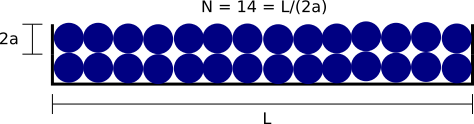
\includegraphics[width=.98\linewidth]{./figures/einsteingeometry.png}
  \caption{Einstein's assumption of N = L/(2a) surface particles available for entrainment is equivalent to a 2D conceptual picture of perfect spheres stacked in a perfect cubic structure.}
  \label{fig:surfaceParticles}
\end{wrapfigure}

He considered that the rate of erosion within the control volume should be proportional to the number of particles available for entrainment and the probability $p/\tau$ that a particle entrains in a unit of time: 
$$ E \propto \frac{L}{a}\frac{p}{\tau}. $$

Of course, mass conservation requires sediment transport is governed by the difference between entrainment and deposition: 
$$ \frac{\partial q_s}{\partial x} = E - D. $$
When transport is in equilibrium, one steady state solution to this differential equation is 
$$ E = D.$$

Einstein considered that the deposition rate of particles $D$ should depend on the sediment transport rate and the particle volume, since particle volume will control the forces on particles, and the sediment transport rate will control the number of particles available for deposition. One dimensionally consistent combination is 
$$ D \propto \frac{q_s}{a^3}.$$
Therefore, using the relations for $E$ and $D$ just assembled, 
$$ q_s \propto a^3 E \propto \frac{L}{2}\frac{a^2}{\tau} p. $$ 

Now the entrainment rate per unit area is expressed in terms of the relevant scales and the entrainment probability $p$. 
One scale which is ambiguous in meaning is the size of the Eulerian control cell $L$. Einstein stated that the most reasonable choice for the control cell size $L$ should be the mean travel distance. 

As in his 1937 work, \textit{travel distance} is intended to mean the summation of individual hop distances over the possible switching combinations between motion and rest, and this is the step in which is 1937 work is at least partially carried forward. 
If the particle travels distance $l$ in each hop as assumed, and the entrainment probability into a hop is $p$, so that the deposition probability from a hop is $1-p$, the mean travel distance will be 
$$ \overline{l} = \sum_{n=0}^{\infty} (1-p)p^n(1+n)l = \frac{1}{1-p} l.$$ 
The reasoning here is that a fraction $1-p$ of particles in motion deposit after traveling distance $l$, while a fraction $(1-p)^2p$ of particles deposit after traveling distance $2l$.
Generalizing, a fraction $(1-p)p^n$ deposit after traveling a distance $(n+1)l$, so that the mean travel distance is the weighted sum above. 

Therefore, Einstein's sediment transport rate is 
$$ q_s = A \frac{p}{1-p} \frac{a^2}{\tau}. $$ 
The constant of proportionality and exchange time scale are its calibration parameters. 

A huge body of work within the stochastic sediment transport literature has been focused on deriving the entrainment probably per unit time $p/\tau$. 

Eistein himself considered that the probability $p$ should be proportional to the interval of time in which the instantaneous lift force surpassed the weight of a bed particle. 
Many investigators followed up this topic and it has been beaten to death \citep{Grass1970, Paintal1969, Paintal1971} etc 

He also prescribed that $\tau$ should be proportional to the particle sedimentation velocity. This is a reasonable assumption of a characteristic velocity scale of particle exchange, but it has been viewed as total conjecture with no empirical evidence available to support or refute this prescription. 

Einstein assumed the exchange time-scale would be related to the particle radius and its sedimentation velocity. Einstein and subsequent researchers did not offer much justification for this assumption. \citep{Cheng2004} and \citet{Paintal1971} employed the bed shear velocity to develop this timescale.

There have been generalizations. 

How is this markov? As presented here this theory is obviously phenomenological and heuristic. 
Einstein's physical and mechanical reasoning is clearly evident reading the original work, but the arguments leading to $q_s$ certainly lack rigor or much clear foundation in earlier work. 

One especially surprising characteristic of the $q_s$ equation is that it does not explicitly contain the velocity of the fluid. 
\citet{Ancey2008} identified this discrepancy and ammended Einstein's theory using the Markov birth-death process. 
They obtain a very similar $q_s$ except that it is explicitly dependent on fluid velocity. 
Also Einstein did not explicitly derive a distribution of sediment transport rates $q_s$. Ancey does this using birth-death processes. 
This work will be reviewed at some point in this thing. 
